\documentclass[tikz,border=3.14pt]{standalone}
\usetikzlibrary{calc}
\begin{document}
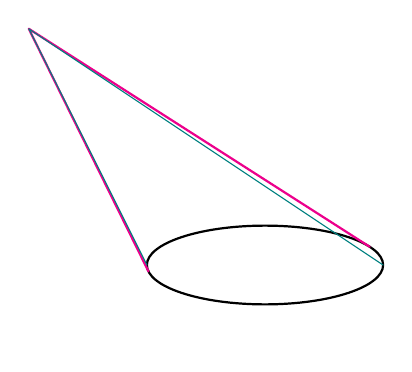
\begin{tikzpicture}[line cap=round,line join=round,thick]
  \def\a{1.5} 
  \def\b{0.5}
  \path (-\a,0) coordinate (A)
        (\a,0)  coordinate (B)
        (-3,3)  coordinate (C);
  \node[circle, minimum size=2cm, outer sep=0pt] (u) {};
  \coordinate (Cp) at ({-3/\a},{3/\b});
  \path (tangent cs:node=u, point={(Cp)}, solution=1) coordinate (T1p);
  \path (tangent cs:node=u, point={(Cp)}, solution=2) coordinate (T2p);
  \path let \p1=(T1p), \p2=(T2p) in
        coordinate (T1) at ({\a*\x1},{\b*\y1})
        coordinate (T2) at ({\a*\x2},{\b*\y2});
  \draw (0,0) ellipse[x radius=\a cm, y radius=\b cm];
  \draw[magenta] (T1) --  (C) -- (T2);
  \draw[teal,thin] (A) --  (C) -- (B);
\end{tikzpicture}
\end{document}
